\section{Oscilador}

En esta sección se analizará el oscilador implementado. La topología propuesta por la cátedra se corresponde con:

\begin{figure}[H]
  \centering
  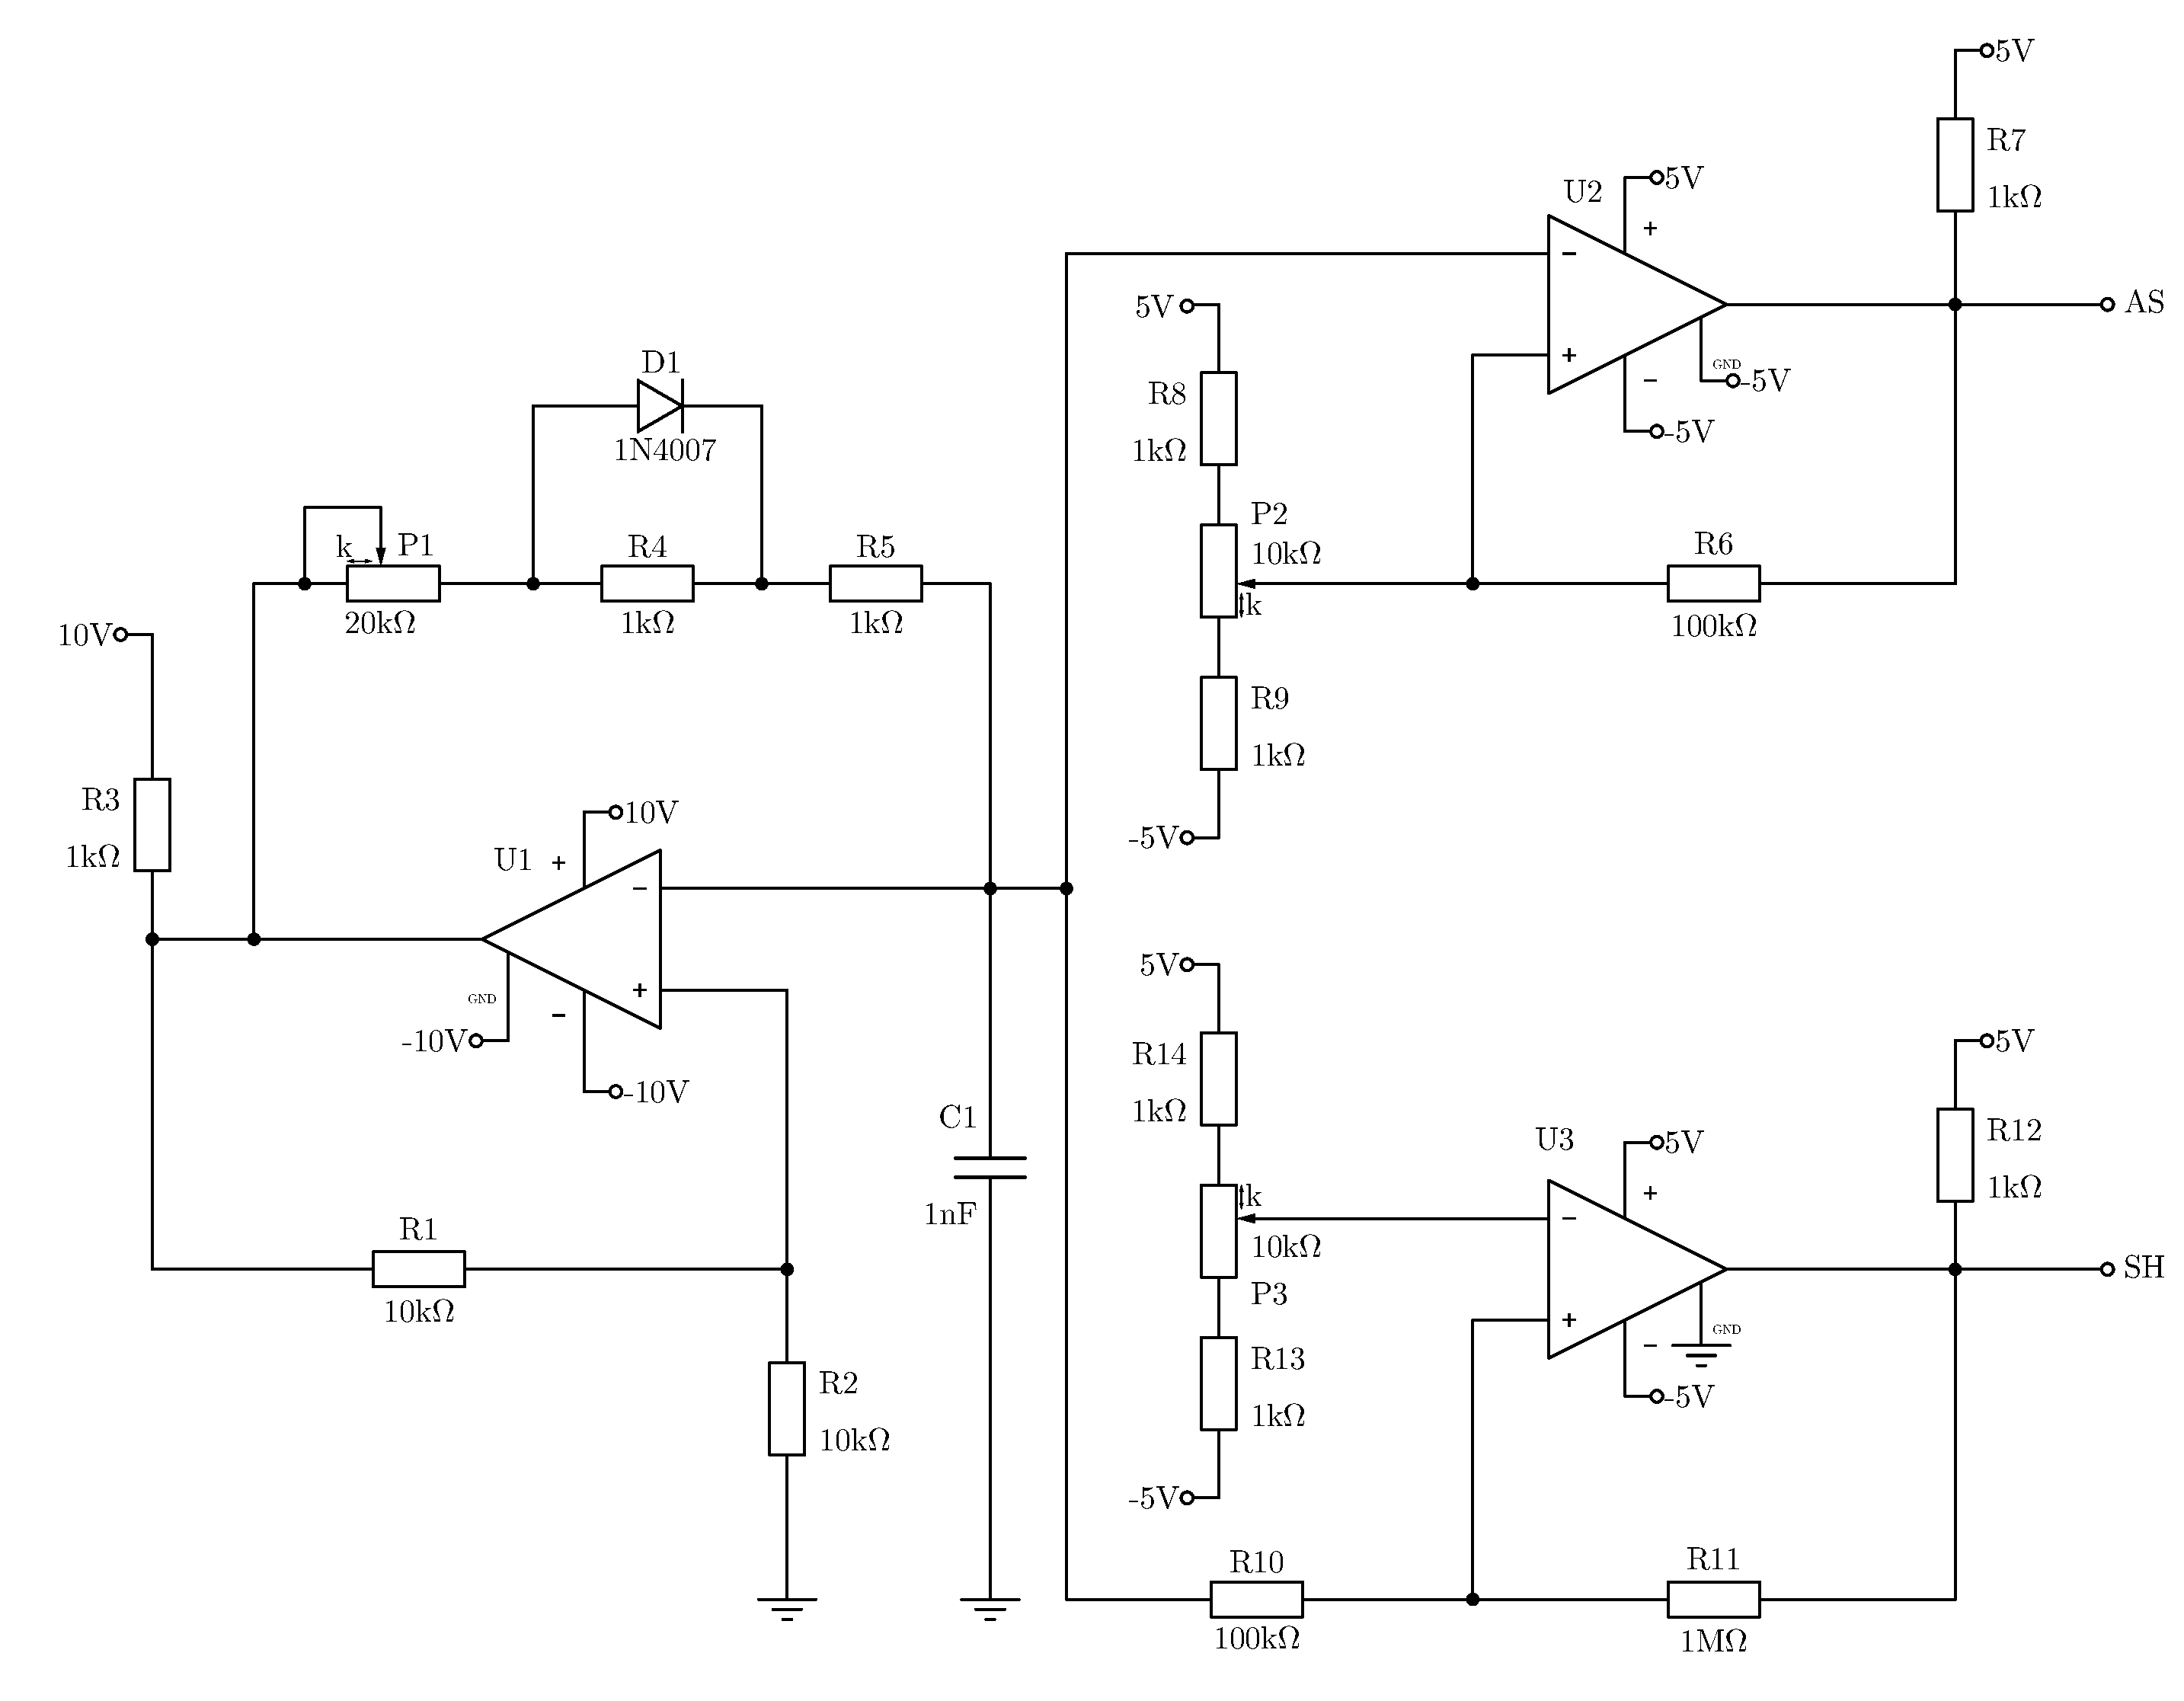
\includegraphics[width = \textwidth]{Imagenes/2_Oscilador/oscilador.pdf}
  \caption{Oscilador propuesto.}
  \label{fig: oscilador}
\end{figure}

\noindent donde es posible analizar al sistema en función de dos partes elementales:

\newpage
\subsection{Oscilador de relajación}

En primera instancia es posible desarrollar el oscilador de relajación presente en el circuito:


\begin{figure}[H]
  \centering
  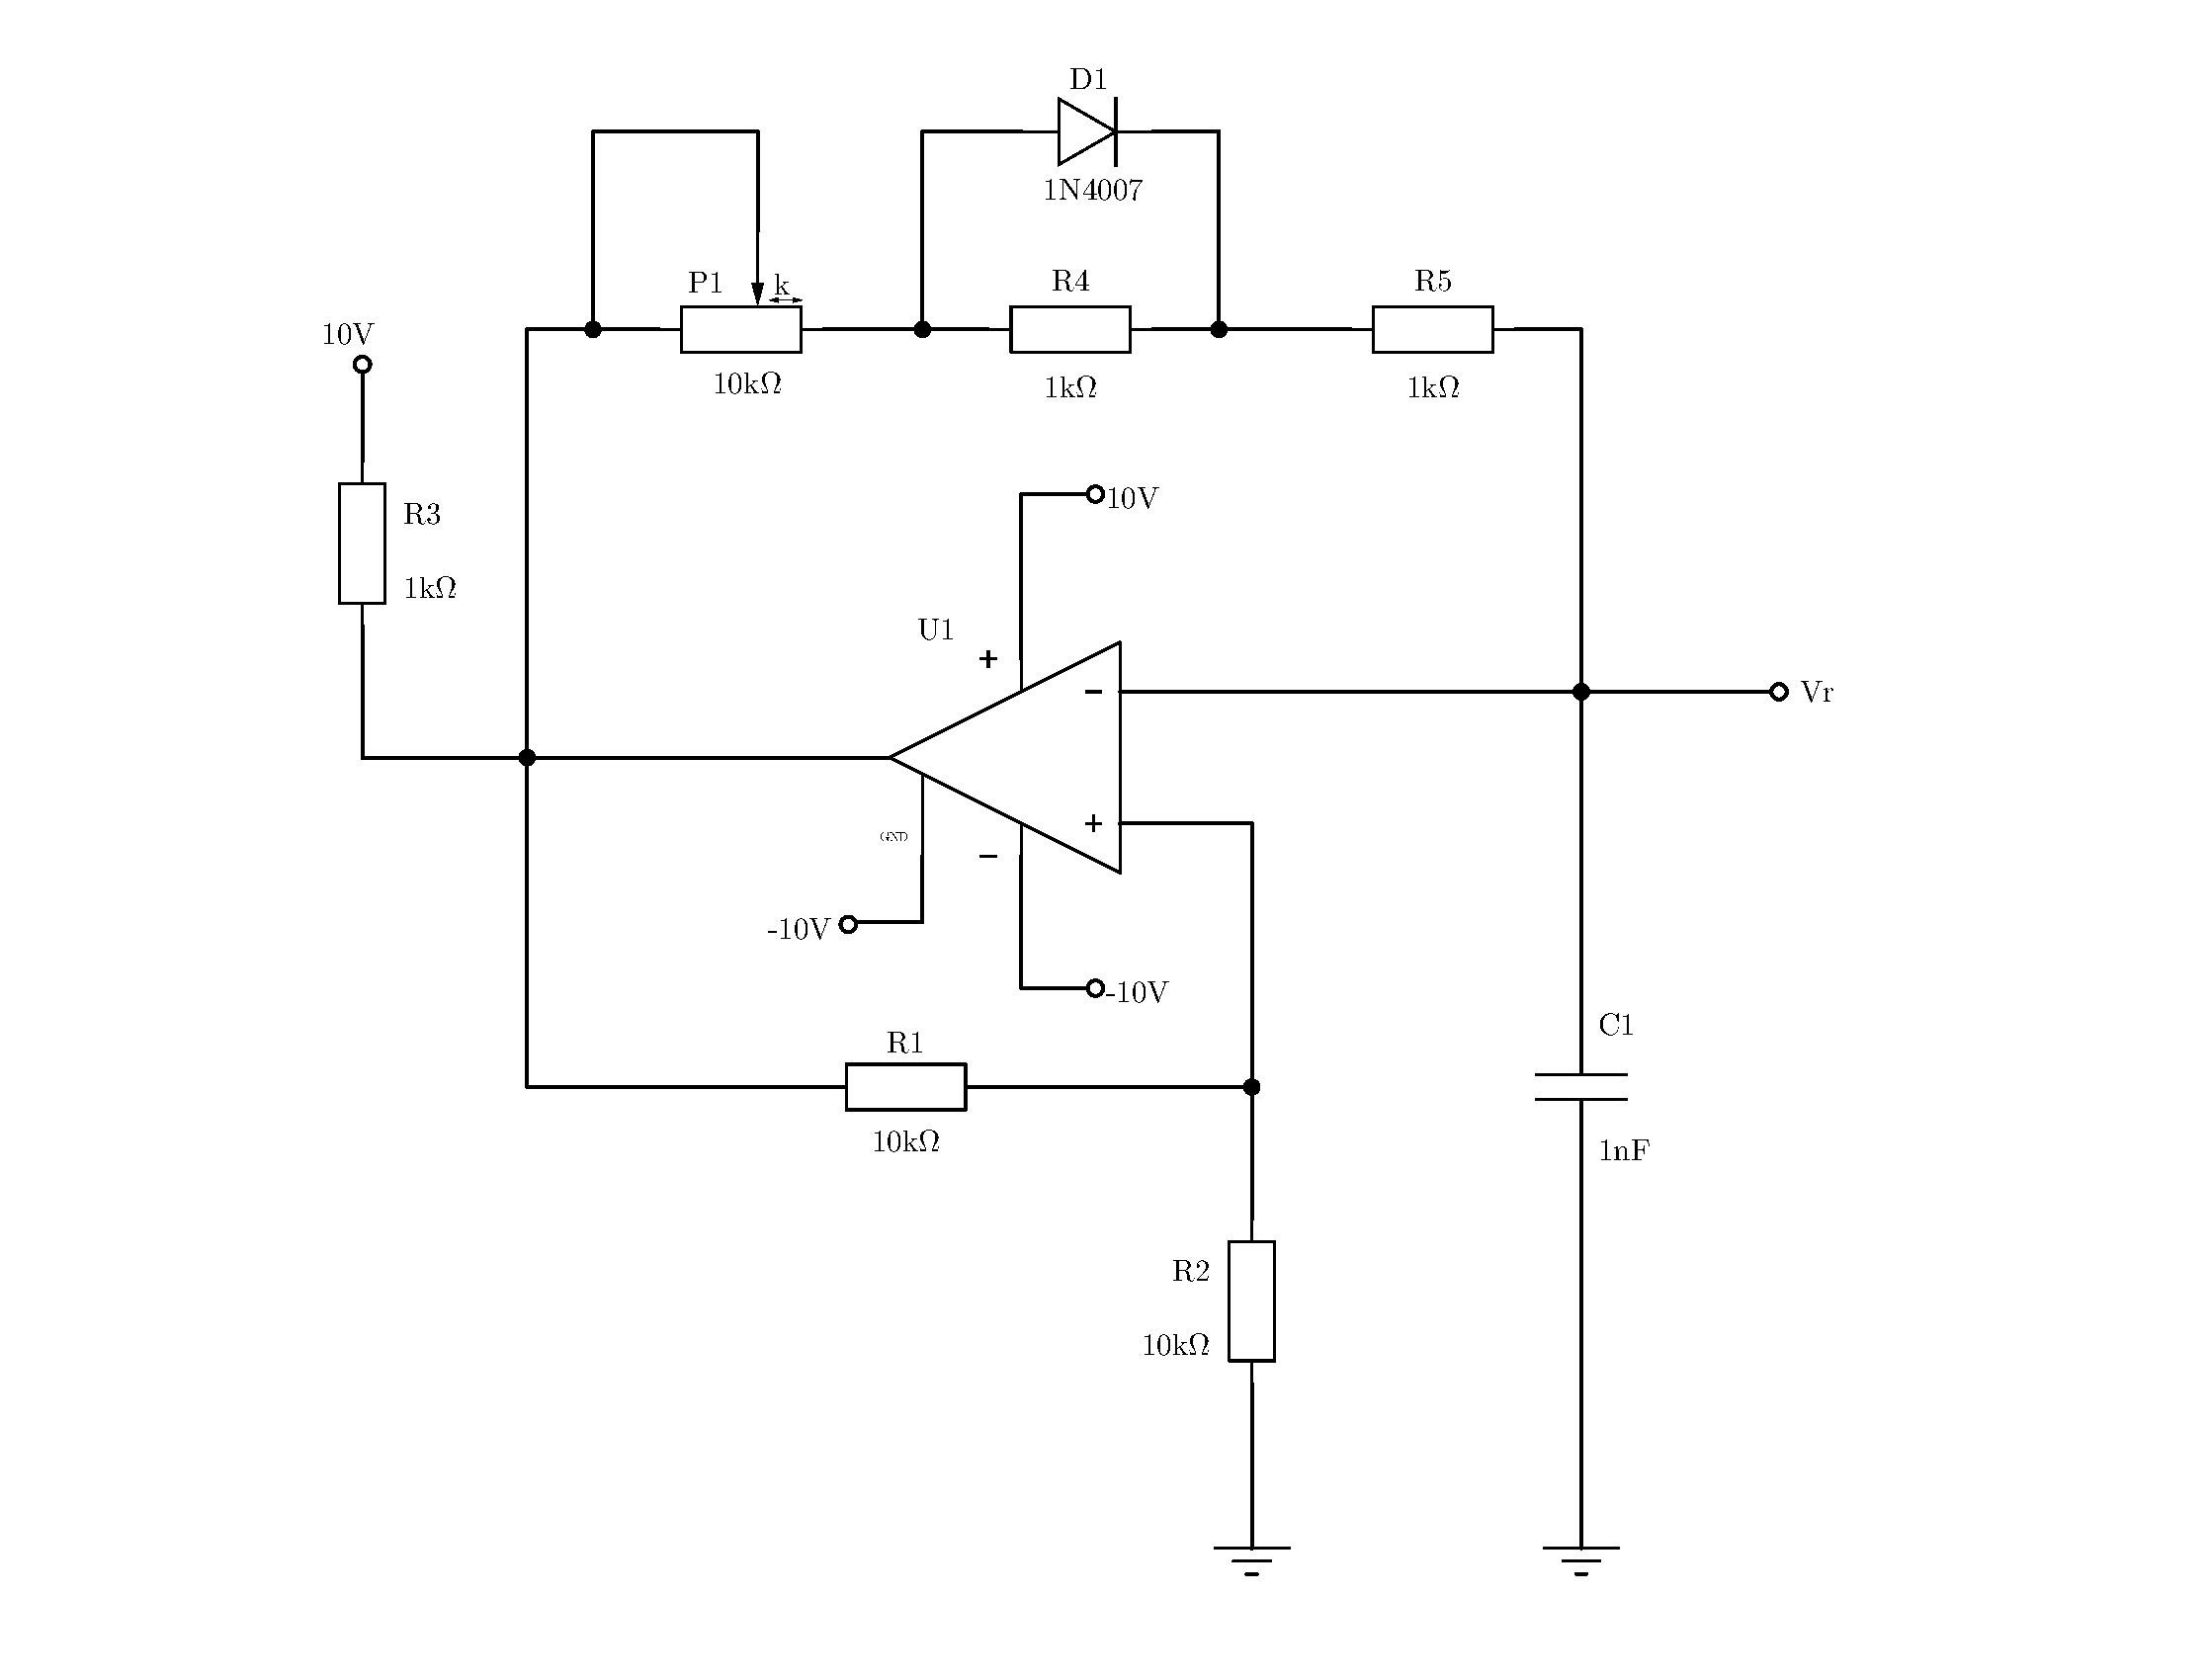
\includegraphics[width = 0.7\textwidth]{Imagenes/2_Oscilador/oscilador_de_relajación.pdf}
  \caption{Oscilador propuesto | Oscilador de relajación.}
  \label{fig: oscilador de relaj}
\end{figure}

\noindent Para comenzar el análisis se puede partir de los valores de tensión que puede tomar la salida del comparador: $\pm 10V$ (en concordancia con los -10V conectados al emisor del comparador y la resistencia de \emph{pull-up} conectada a 10V). En función de este hecho, la tensión en la entrada no inversora del comparador puede ser $\pm 5V$ respectivamente.

Una vez que se definieron los posibles niveles de comparación en la entrada no inversora y los posibles valores que toma la salida del comparador, es posible analizar la dinámica del nodo $V_r$ en función de la respuesta al escalón de los circuitos:

\begin{figure}[H]
    \centering
    \begin{subfigure}{0.48\textwidth}
        \centering
        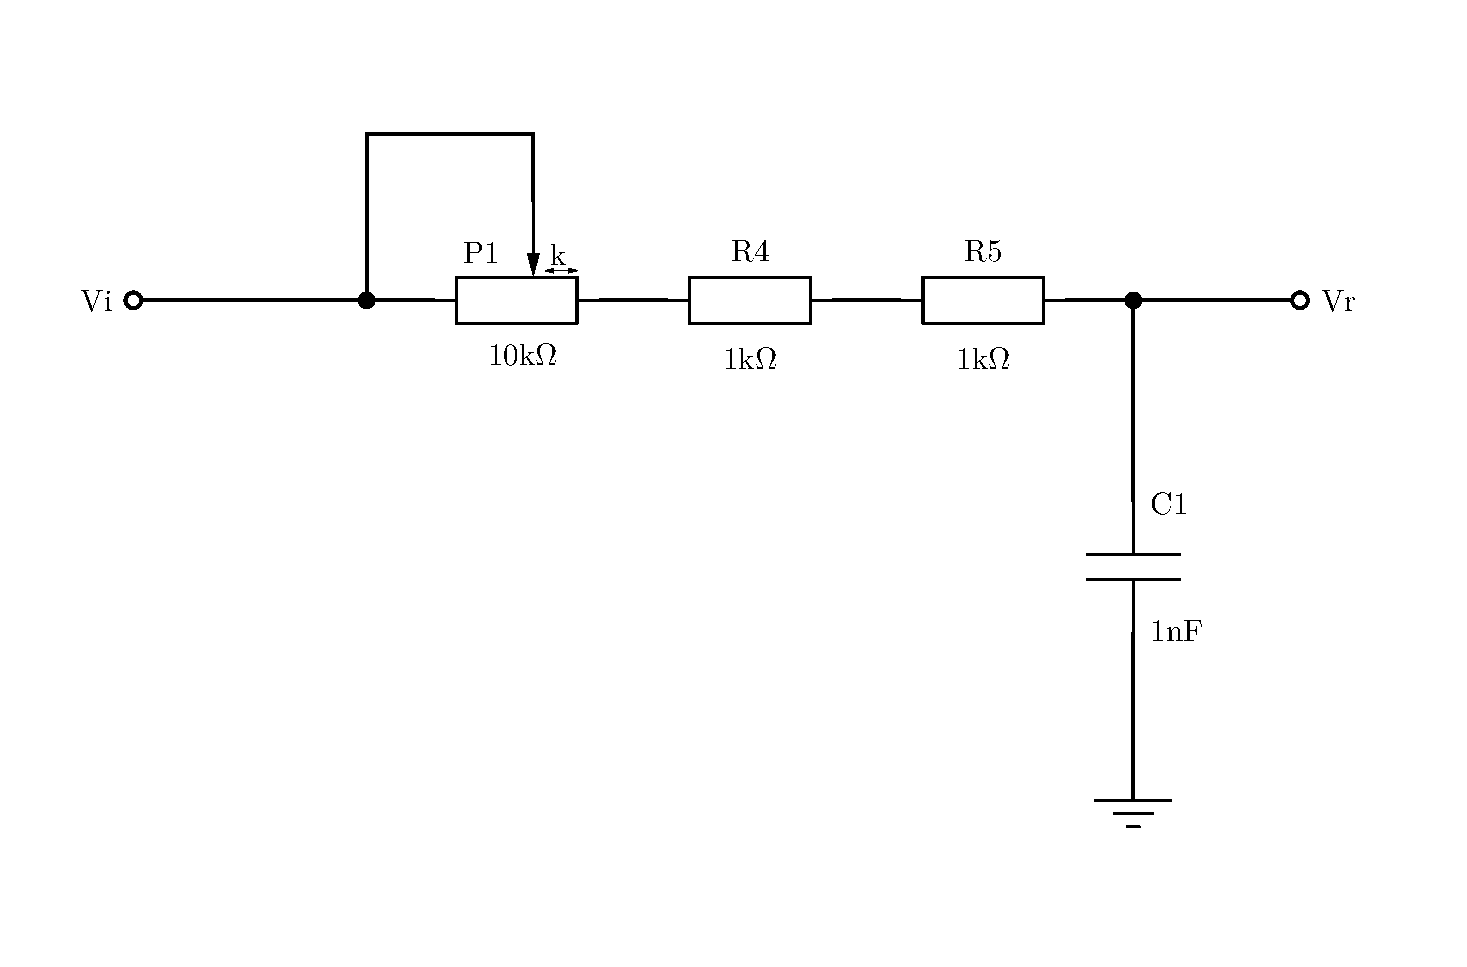
\includegraphics[width=\textwidth]{Imagenes/2_Oscilador/osc_rel_neg.pdf}
        \caption{Sistema en flanco ascendente.}
        \label{fig: sistema en flanco ascendente}
    \end{subfigure}
    \hfill
    \begin{subfigure}{0.48\textwidth}
        \centering
        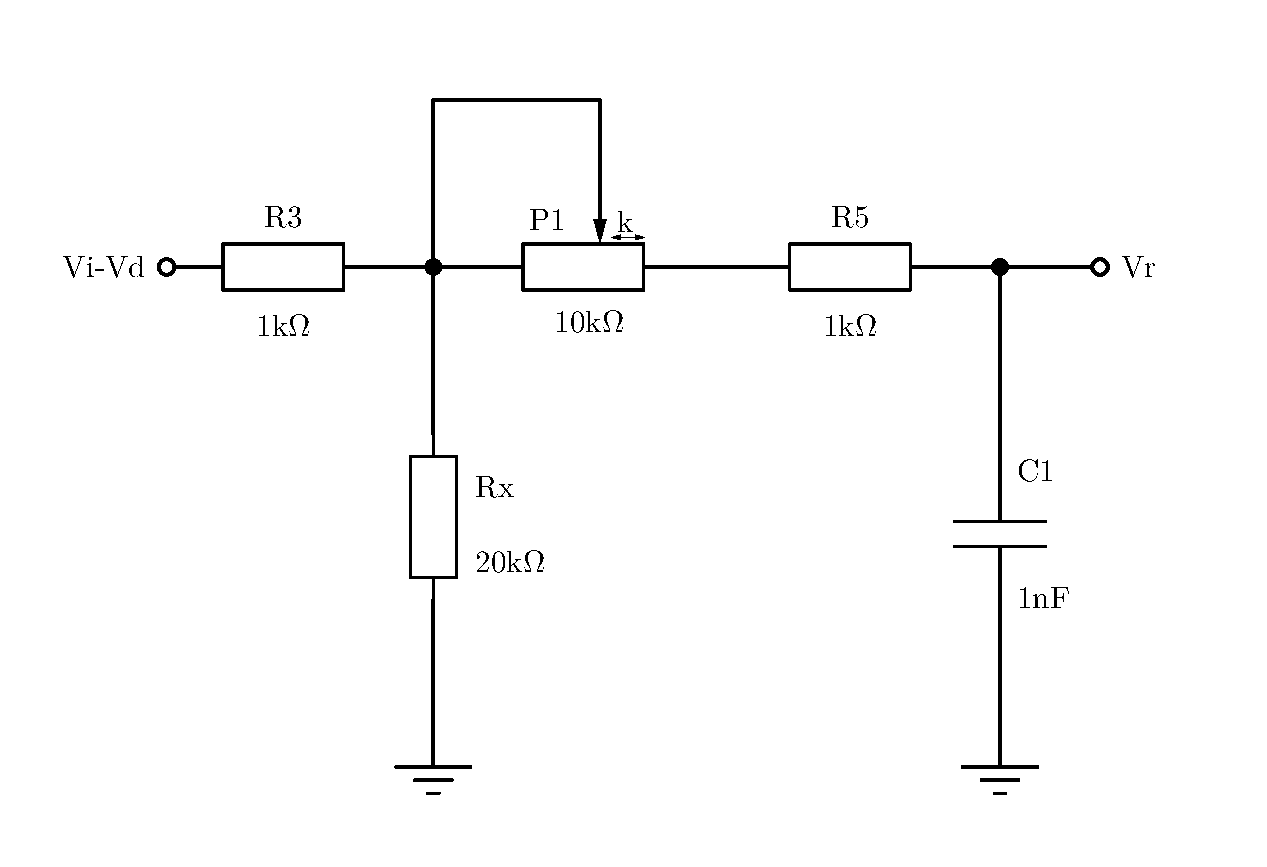
\includegraphics[width=\textwidth]{Imagenes/2_Oscilador/osc_rel_pos.pdf}
        \caption{Sistema en flanco descendente}
        \label{fig: sistema en flanco descendente}
    \end{subfigure}

    \caption{Circuitos a analizar respuesta al escalón.}
    \label{fig: circuitos a analizar rta al escalón}
\end{figure}

De este modo, la respuesta del sistema sera:

\begin{align*}
    a_{(t)} = A \cdot (1 - e^{-t/\tau})
\end{align*}

Si se toma como condición inicial la situación donde la entrada inversora alcanza los $5V$ y la salida del comparador transiciona de $10V \rightarrow -10V$, se está analizando el flanco descendete del sistema. De este modo, estamos analizando la respuesta a un escalón de altura $A = -10V-5V=-15V$ sobre el circuito \ref{fig: sistema en flanco descendente}. En este contexto:

\begin{equation}
    \tau_{des} = (1k\Omega + 0.95k\Omega + k \cdot 10k\Omega) \cdot 1nF = 1.95\mu s + k \cdot 20\mu s
\end{equation}

De este modo es posible calcular el tiempo en el que se produce este flanco, considerando que la comparación se realiza contra $-5V$, por lo que en el:

\begin{align*}
    &(-15V) \cdot (1 - e^{-t_-/\tau_{des}}) = -10V \\
\Longrightarrow \: & e^{-t_-/\tau_{des}} = 1 - \frac{10V}{15V} \\
\Longrightarrow \: & t_- = -(1.95\mu s + k \cdot 20\mu s) \cdot ln\left(1 - \frac{10V}{15V}\right)
\end{align*}

\noindent de este modo  $ 2,14\mu s< t_- <26,376\mu s$


